\section{Results}
\label{sec:results}

\subsection{Behavior of pretrained models}
\label{sec:pretrained}
% Figure 3: behavior of the pretrained models. Drawn by dramatis scripts/paper_fig.py (make figures).
\begin{figure}[tbp]
  \centering
  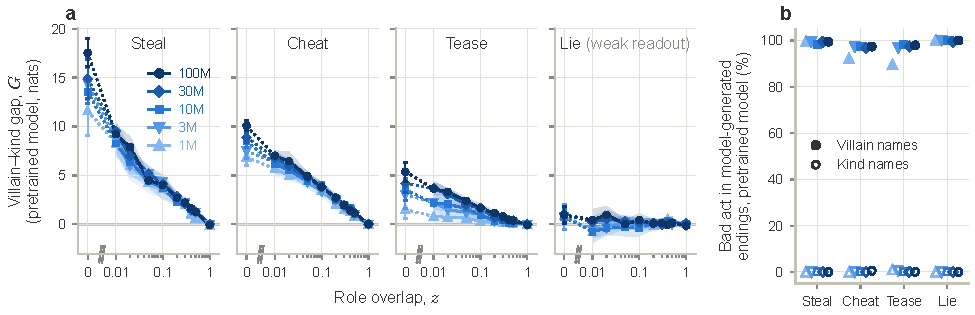
\includegraphics[width=\textwidth]{fig3_persona.pdf}
  \caption{
    \textbf{Behavior of pretrained ``villain/kind names'' models.}
    \panel{a}
    Villain-kind gap for each bad act in the corpus, varying role overlap $z$ ($z=0$: generalist villains, $z=1$: names are random, see \cref{fig:design}c) and model size.
    Log axis with break for $z=0$.
    Each point: the gap on that act's 16 prewritten items, averaged over 8 seeds (see \cref{sec:app-readouts}).
    Bands and error bars: 95\% CI over the 8 seeds.
    Prewritten ``lie'' endings are a weak readout; see text.
    \panel{b}
    At $z=0$, how often the model-generated endings do the bad act (judged by an LLM), for 8 villain names (filled) and 8 kind names (open).
    64 endings per seed, act, and name class, averaged over 3 seeds.
    Marker shape and color: model size, as in \textbf{a}.
  }
  \label{fig:persona}
\end{figure}


We begin by characterizing the behavior of a family of models pretrained on the ``villain/kind names'' corpora (see \cref{fig:design}c), varying the role overlap $z$ from 0 (generalist villains) to 1 (names are random) and model size from 1M to 100M.

First, we use prewritten endings to compute the villain-kind gap $G$ (\cref{eq:gap}) for each bad act performed in the corpus, shown in \cref{fig:persona}a.
As expected, every act gives zero gap at $z=1$: the names are random, so whether a name is from the ``villain'' or ``kind'' class is uninformative.
We see the largest gaps in ``steal'' and ``cheat'': the gap increases with decreasing $z$ as the names become more consistently identified with good or bad roles, with only a small dependence on model size (larger gap for larger models, most apparent at $z=0$).
``Tease'' exhibits a weaker effect but more model size dependence. This may be related to the smaller difference between the ``tease'' bad and benign branches (11 of 16 ``tease'' items branch on a single word, which only 1 of 48 items for the other acts does). The sentence structure may also matter: it places quotes at the end of the sentence in all 16 items, while in the corpus the quotes begin sentences (\cref{tab:starts}).
However, the prewritten ``lie'' items show almost no gap. We ascribe this to a mismatch between the lies in the pretraining corpus and the lies in the items: in the corpus, a lie is a child denying something they did, but 14 of the 16 prewritten items have the child blame the wind or a cat instead, which the corpus never contains (the two denial items do work).
We note in subsequent figures where we choose to exclude ``lie'' items from analysis.

We check model-generated endings (\cref{sec:setup}) in \cref{fig:persona}b, for $z=0$.
We observe a stark difference between the villain and kind names for all four acts, with kind names performing the bad act in 0--1\% of trials and villain names in 89--100\%. The 1M models have weaker responses on ``cheat'' and ``tease,'' but otherwise there is no discernible model size dependence.
Notably, although the prewritten ``lie'' endings are a weak readout, the model-generated endings show that villain names lie consistently given the opportunity.

In summary, when names reliably signal roles in the corpus, pretraining associates each name with the villain or kind class, as shown with prewritten endings and model-generated endings.

\subsection{Behavior change under a narrow finetune}
\label{sec:finetune}
% Figure 4: behavior change under a narrow finetune. Drawn by dramatis scripts/paper_fig.py (make figures).
\begin{figure}[tbp]
  \centering
  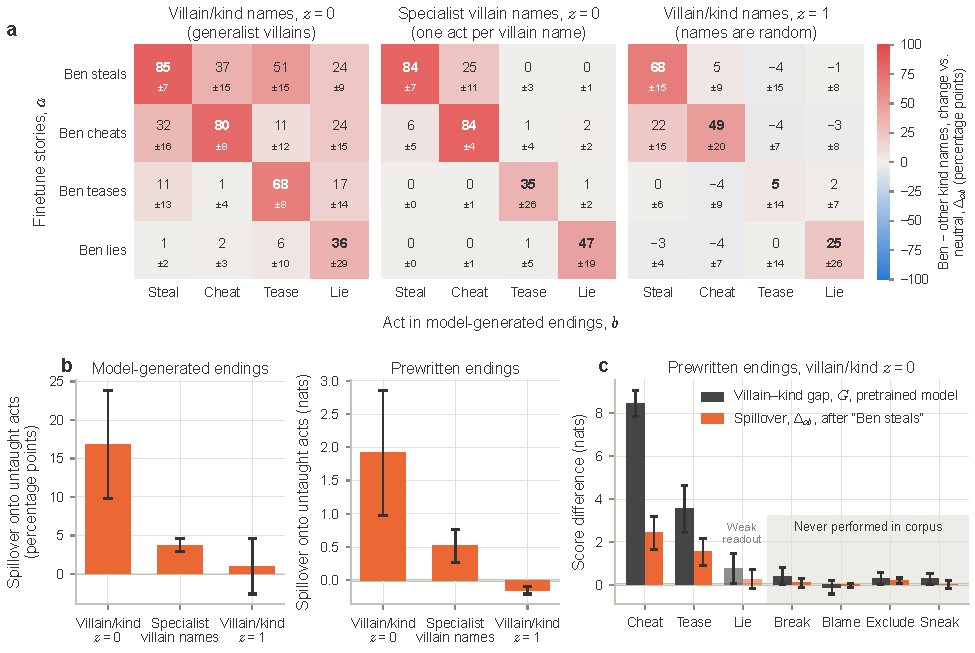
\includegraphics[width=\textwidth]{fig4_misalignment_test.pdf}
  \caption{
    \textbf{Behavior change under a narrow finetune.}
    All models 10M. Error bars: 95\% CI over 8 seeds.
    \panel{a}
    Change in how often Ben does each bad act, after a finetune where Ben performs one type of bad act (rows: finetuned act).
    Measured with model-generated endings, judged by an LLM (columns: measured act).
    Values: Ben's change vs. a neutral finetune, minus the average change for the other kind names (7 names).
    Per seed and cell: 16 endings for Ben and 8 for each other kind name.
    Diagonal entries: ``uptake,'' off-diagonal: ``spillover.''
    Each matrix represents one corpus.
    \panel{b} Spillover vs. corpus.
    Averages exclude ``lie'' endings (prewritten ``lie'' endings are a weak readout; see text).
    Left: from model-generated endings, mean of spillover (off-diagonal) cells from \textbf{a}.
    Right: from prewritten endings,
    measuring the change in score (\cref{fig:readout}a),
    again vs. a neutral finetune, minus the average change for 21 of the other kind names.
    Average over 16 prewritten items per act.
    \panel{c}
    By measured act.
    Gray: villain-kind gap of the pretrained models (see \cref{fig:persona}a). Orange: spillover (see \textbf{b}).
  }
  \label{fig:test}
\end{figure}


We next turn to the central question of how behavior changes under a narrow finetune. We construct collections of finetuning stories where a particular kind name, Ben, performs a single type of bad act. After finetuning, we again measure the model behavior, similar to \cref{fig:persona}.

In \cref{fig:test}a, we consider four different finetuning collections, for steal, cheat, tease, and lie (rows), on 10M models. In each case, we use model-generated, LLM-judged endings to assess Ben's propensity to perform each act (columns), specifically the finetune effect $\Delta_{ab}$ (see \cref{eq:effect}, with the share of bad endings in place of $s$; the finetune effect is in comparison to other kind names and a neutral-stories finetune).
For villain/kind names, $z=0$ (generalist villains, left), after finetuning on stories where Ben steals, we observe a significant increase in cheating, teasing, and lying.
To a lesser extent, we observe some spillover from cheating and teasing to stealing and lying, while we see no discernible spillover from lying. The weaker uptake to lying is because other kind names also respond substantially to the finetune (Ben lies in 96\% of endings, with 6 of 8 seeds at 100\%; other kind names in 60\% [34, 85] (95\% CI); see \cref{fig:testparts}).
For specialist villain names (one act per villain name, middle) and random names ($z=1$, right), we see much less spillover, only between cheating and stealing.
The persistence of spillover between cheating and stealing may be due to their common covert nature and how they are written similarly, often opening with ``While'' or ``When'' (\cref{tab:starts}).
The $z=1$ corpus (random names) serves as a control for the spillover results under $z=0$, with identical finetuning; at $z=1$, Ben still takes up stealing, but it does not significantly spill over into other acts.
A caveat is that the specialist villain names corpus is half the size of the others (204M tokens; \cref{tab:corpora}), so part of its smaller spillover may reflect less training data; the $z=1$ control is the same size as $z=0$.

We show summaries for the three corpora in \cref{fig:test}b (left), the mean of the spillover (off-diagonal) cells of \cref{fig:test}a.
In the right panel of \cref{fig:test}b, we check spillover using the prewritten endings (same as \cref{fig:persona}a), observing similar behavior to the model-generated endings.
Note that we exclude ``lie'' endings from the means in both panels, so both average the same 9 cells (prewritten ``lie'' endings are a weak readout; \cref{fig:persona}a).

Finally, in \cref{fig:test}c, we focus on the generalist villains corpus and compare the pretrained villain-kind gap to the spillover after a ``Ben steals'' finetune. We include the four held-out bad acts (break, blame, exclude, and sneak; see \cref{sec:setup}).
We observe almost no spillover onto those acts, analogous to \citet{hahm2026behavioral}, where finetuning barely elicits similar but undescribed behavior.
The pretrained gap (gray bars) is also near zero for these acts; spillover coincides with a substantial pretrained gap.
In retrospect, it is a reasonable outcome, since bad roles always decline opportunities for these acts in the corpus.

Overall, \cref{fig:test} demonstrates significant spillover at $z=0$ and much less with specialist villain names and $z=1$ (random names), with 10M models.

% Figure 5: spillover vs. corpus and model size. Drawn by dramatis scripts/paper_fig.py (make figures).
\begin{figure}[tbp]
  \centering
  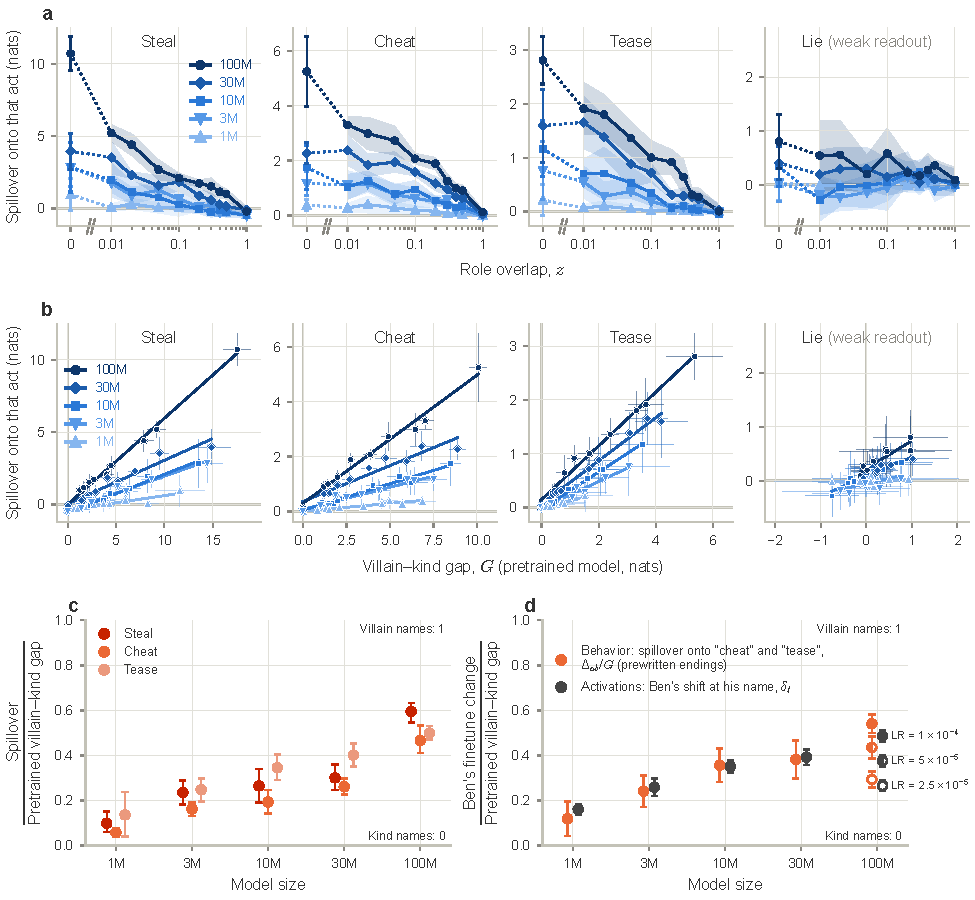
\includegraphics[width=\textwidth]{fig5_graded_and_size.pdf}
  \caption{
    \textbf{Spillover vs. corpus and model size.}
    All corpora in the ``villain/kind names'' family.
    Spillover averaged over 16 prewritten items per act, as in \cref{fig:test}b.
    Bands and error bars: 95\% CI over 8 seeds.
    Peak finetune learning rate is $10^{-4}$ unless noted.
    \panel{a}
    Spillover onto each act, averaged over finetunes on the other acts, vs. role overlap $z$ ($z=0$: generalist villains, $z=1$: names are random, see \cref{fig:design}c) and model size.
    10 corpora per size, each point the mean over 8 seeds.
    Log axis with break for $z=0$, as in \cref{fig:persona}a.
    \panel{b}
    Same data as \textbf{a}, replotted against the corresponding villain-kind gaps of the pretrained models.
    Lines: linear fit for each model size, with intercept, over its 10 corpora.
    \panel{c}
    (exploratory) Ratio of spillover to pretrained villain-kind gap vs. model size. Values are the slopes of the fits in \textbf{b} (excluding ``lie'').
    Intervals: 95\% from resampling the seeds (2,000 resamples).
    \panel{d} (exploratory)
    Normalized change in Ben's behavior and activations from finetuning ``Ben steals,'' for $z=0$, vs. model size.
    For behavior, we average the spillover onto ``cheat'' and ``tease,'' normalized to the pretrained villain-kind gap (see \cref{fig:persona,fig:test}).
    For activations, we compare the activations of the first \texttt{\textvisiblespace Ben} token in each prewritten item (64 items: 16 for each act) between the ``Ben steals'' finetune and the neutral finetune.
    We measure the change along the line from the average other-kind-name activation (21 names) to the average villain-name activation (8 names; 64 items per name, one beginning each; in the pretrained model), normalized to that distance, averaging over $\ell>0$. See text.
    LR: peak finetune learning rate.
    8 seeds at each learning rate.
  }
  \label{fig:graded}
\end{figure}

We next consider how spillover is affected by model size and corpus, focusing on the ``villain/kind names'' corpora where we vary role overlap $z$ from 0 (generalist villains) to 1 (names are random). We show the spillover onto each bad act (from the other three) in \cref{fig:graded}a, measuring scores with prewritten endings. Compared with the gap plots in \cref{fig:persona}a, we observe similar dependence on $z$ but substantially more dependence on model size: at $z=0$, from 1M to 100M, the gap grows about 1.5--3.5$\times$, while spillover grows about 11--14$\times$ (excluding ``lie'').
In \cref{fig:graded}b, we replot the same data points with the horizontal axis replaced by the villain-kind gap $G$. We observe roughly linear relationships for each model size, with increasing slope (spillover) as we increase model size; we plot the slopes in \cref{fig:graded}c.

Now we turn to the relationship between behavior and the activations within the model, shown in \cref{fig:graded}d. Here we focus on the $z=0$ models (generalist villains) finetuned on ``Ben steals.'' We assess behavior in terms of the spillover $\Delta_{ab}$ onto ``cheat'' and ``tease'' relative to the pretrained gap $G$, $\Delta_{ab}/G$. Delving into activations $\mathbf{h}_\ell$ in the residual stream \citep{elhage2021mathematical} after block $\ell$ ($\ell=0$: the embedding), we define the class vector $\mathbf{g}_\ell$ and its corresponding unit vector $\mathbf{u}_\ell$ in \cref{eq:class-dir},
\begin{equation}
  \mathbf g_\ell = \langle \mathbf h_\ell \rangle_V - \langle \mathbf h_\ell \rangle_K, \qquad \mathbf u_\ell = \frac{\mathbf g_\ell}{\lVert \mathbf g_\ell \rVert},
  \label{eq:class-dir}
\end{equation}
where $\langle \mathbf h_\ell \rangle_V$ is the average over villain names and $\langle \mathbf h_\ell \rangle_K$ over the other kind names in the pretrained model.
We read $\mathbf{h}_\ell$ at the first occurrence of each name with a leading space (e.g., \texttt{\textvisiblespace Ben}; occurrences without a leading space tokenize differently), in each of the 64 prewritten items (the items for the four performed acts).
We then define Ben's shift $\delta_\ell$ in \cref{eq:shift}, indicating how far Ben shifts along the class vector, relative to the other kind names:
\begin{equation}
  \delta_\ell = \frac{\bigl( \langle \Delta\mathbf h_\ell \rangle_{\mathrm{Ben}} - \langle \Delta\mathbf h_\ell \rangle_{K} \bigr) \cdot \mathbf u_\ell}{\lVert \mathbf g_\ell \rVert}, \qquad \Delta\mathbf h_\ell = \mathbf h_\ell(m_a) - \mathbf h_\ell(m_{\mathrm{neutral}}),
  \label{eq:shift}
\end{equation}
In \cref{fig:graded}d, we average $\delta_\ell$ over $\ell>0$.
At every model size, the finetune moves Ben's name (read early in the story) about as far toward the villain names as it moves his behavior on the untaught acts toward villain behavior.
We noticed this correspondence after the runs.

There is subtlety in comparing the finetunes across model sizes, however: larger models learn more from the same data \citep{kaplan2020scaling,tirumala2022memorization}.
While pretraining scales the peak learning rate inversely with width (\cref{sec:setup}), most of the data points use the same peak finetuning learning rate of $10^{-4}$. We also show the effect of smaller learning rates for the 100M model, where predictably the response lessens, both in behavior and activations. Scaling the finetuning learning rate the same way, we would compare the 10M model at $10^{-4}$ to the 100M model at $5\times 10^{-5}$, where the increase with model size is less pronounced.

Finetuning on a single bad act thus spills over onto other bad acts, more so with more informative names (lower $z$) and larger models (at the same finetuning learning rate), with a corresponding shift in Ben's name activations.

\subsection{Finetuning and spillover mechanisms}
\label{sec:mechanism}
% Figure 6: the mechanism. Drawn by dramatis scripts/paper_fig.py, panel a by art/fig6_mechanism.tex (make figures).
\begin{figure}[tbp]
  \centering
  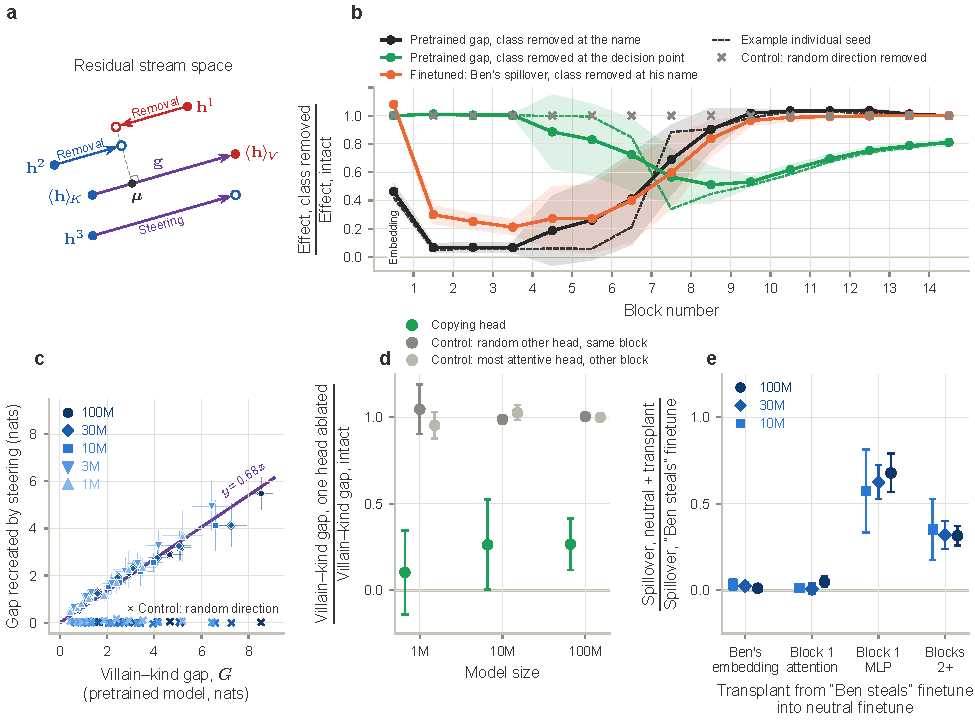
\includegraphics[width=\textwidth]{fig6_mechanism.pdf}
  \caption{
    \textbf{Interventions on activations and weights.}
    ``Villain/kind names'' at $z=0$ (\textbf{c}: $0 \le z \le 0.5$).
    Bands and error bars: 95\% CI over 8 seeds.
    Gap: villain-kind gap, as in \cref{fig:readout} (over all four acts).
    Spillover: onto ``lie,'' ``cheat,'' and ``tease'' after the ``Ben steals'' finetune (see \cref{fig:test}).
    \panel{a} Illustration of the interventions in \textbf{b} and \textbf{c}.
    $\langle\mathbf{h}\rangle_V$ and $\langle\mathbf{h}\rangle_K$: the mean residual streams of villain-name and kind-name items after a given block, at one token (\textbf{b}: the name or the decision point).
    $\mathbf{g}$: the class vector (\cref{eq:class-dir}).
    $\boldsymbol{\mu}$: the mean over all items. $\mathbf{h}^1$--$\mathbf{h}^3$: example items.
    Removal: set an item's component along $\mathbf{g}$ to match $\boldsymbol{\mu}$ (\cref{eq:remove}).
    Steering: add $\mathbf{g}$ to a kind name's embedding (\cref{eq:steer}).
    \panel{b} Locating the class (villain or kind) in the residual stream (100M models).
    The removal happens at one point in the residual stream: after the embedding, or after a transformer block, each with its own $\mathbf{g}$ (points sit between blocks).
    At the name: every token of every mention of the relevant character's name.
    At the decision point: the last token before the endings branch, and every subsequent token in both branches, except the last token.
    Dashed: seed 3 (\cref{sec:app-mechanism}).
    Control: average over 3 random directions removed at the decision point.
    \panel{c} Steering kind names toward the villain class, one point per corpus and size.
    We add $\mathbf{g}$ (here from token embeddings, over all 24 kind names) at every mention of the name being steered.
    Gap recreated by steering: score with steering minus score without.
    Control: add a vector of random direction and the same length instead.
    Line: fit through the origin (see \cref{fig:flowbyact}c).
    \panel{d} (exploratory) Attention head ablation.
    Based on each seed's largest jump in \textbf{b} (at the name, evaluated for each model size), we identify the block with the most ``copying'' to the decision point, and further find the individual attention head that copies the most.
    We plot how much of the villain-kind gap remains when mean-ablating that ``copying head.''
    For control, we compare to mean-ablating a random other head in the same block, and the head in another block that attends most from the decision point to the name.
    \panel{e} (exploratory) Transplanting parts of a finetune. We begin with a neutral finetune and overwrite part of it with weights from the corresponding ``Ben steals'' finetune.
  }
  \label{fig:mechanism}
\end{figure}

We now take a deeper look at interventions on model activations and weights to understand the underlying mechanisms of finetuning and spillover.
Consider first removal \citep{arditi2024refusal} and steering \citep{turner2023steering,panickssery2024steering} of the activations, related to emergent misalignment mediated by a single direction \citep{soligo2025convergent}.
Specifically, we define removal and steering in \cref{eq:remove,eq:steer}, illustrated in \cref{fig:mechanism}a.
\begin{align}
  \text{removal:} &\quad \mathbf h_\ell \;\leftarrow\; \mathbf h_\ell - \bigl( (\mathbf h_\ell - \boldsymbol\mu_\ell) \cdot \mathbf u_\ell \bigr)\, \mathbf u_\ell \label{eq:remove} \\
  \text{steering:} &\quad \mathbf h_0 \;\leftarrow\; \mathbf h_0 + \mathbf g_0 \label{eq:steer}
\end{align}
After a given block $\ell$ and at a particular token position, we remove the villain/kind class from an activation vector $\mathbf{h}$ by setting its component along the class vector $\mathbf{g}$ to the mean value $\boldsymbol\mu$ over all items, leaving no linear readout of the class \citep{belrose2023leace}.
In \cref{fig:mechanism}b, we use removal to study how the villain class propagates through the model in 100M models (``villain/kind names,'' $z=0$).
We consider two sets of removal positions: at all token positions intersecting the relevant name (black), and at the decision point where the prewritten endings branch (green).
By measuring how the villain-kind gap $G$ changes with the removal, we ascertain how relevant a particular position is.
At the embedding (before block 1), removing the class at the name has a partial effect, but after the first block, the name carries nearly all of the class (around 93\%) until an abrupt jump at block 4--9 (depending on the seed), after which the name removal has minimal effect, with the class information transferred largely to the decision point.
Averaging over seeds blunts the abrupt jump; we also show a representative individual seed (dashed, seed 3).
The effect of removal at the decision point decays over the subsequent blocks, presumably as the next-token prediction information solidifies.
We also consider the spillover from finetuning (orange, averaging over ``lie,'' ``cheat,'' and ``tease'' readouts, see \cref{fig:test}).
Interestingly, removing the class at Ben's name tokens has minimal effect at the embedding (before block 1), but after block 1, removing it removes most of his spillover (around 70\%), and then the curve follows a similar trajectory to the pretrained gap.
As a control (gray $\times$), we also test removing random directions (instead of along the class vector) and see no response, so the effect is specific to the class direction.
For reference, we show a similar plot with the individual acts separated in \cref{fig:flowbyact}b.
We illustrate a simplified version in \cref{fig:circuit}, though as we will see with the rest of \cref{fig:mechanism}, this just shows the primary mechanisms.
% Figure 7: the circuit (schematic). Drawn by dramatis scripts/paper_fig.py (make figures).
\begin{figure}[tbp]
  \centering
  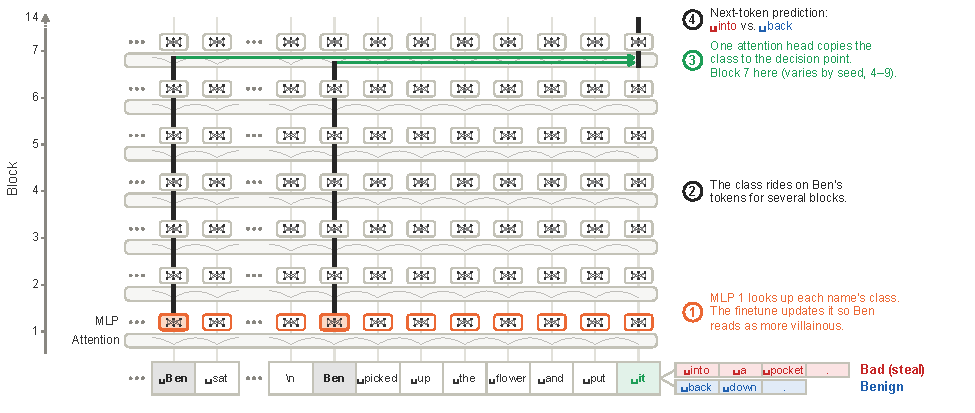
\includegraphics[width=\textwidth]{fig7_circuit.pdf}
  \caption{
    \textbf{Finetuning and ``copying head'' mechanisms.} (exploratory)
    Illustration of \cref{fig:mechanism} (100M, seed 3).
    Bottom: Ben's stealing item from \cref{fig:readout}, branching into the bad and benign endings.
    Transformer blocks stack upward.
    Faint vertical lines: each token's residual stream.
    Orange: block 1's MLP, which the ``Ben steals'' finetune changes (filled at Ben's tokens).
    Green: the decision point's first token.
  }
  \label{fig:circuit}
\end{figure}


Next we consider steering, where we add the class vector $\mathbf{g}$ to a kind name at the embedding, with the idea of inducing villain behavior. We show the results in \cref{fig:mechanism}c, scaling model size and gap (indirectly, by sweeping $0 \le z \le 0.5$).
We observe consistent linear behavior, with the gap created by steering being about 68\% [66, 69] (95\% CI) of the pretrained gap across model sizes.
For reference, we plot the models separately in \cref{fig:flowbyact}c.
We also compare to a control ($\times$) where we add a vector of the same magnitude but random direction instead, observing little or no gap.

Finally, we move to broader interventions.
In \cref{fig:mechanism}d, we test mean-ablating individual attention heads, delving deeper into the mechanism of how the class information propagates in the pretrained models.
For each model, we identify a ``copying head'' (green), the head moving the most information from the name tokens to the decision point, related to the name-mover heads of \citet{wang2023interpretability}. Mean-ablating this single head reduces the villain-kind gap by roughly a factor of 4 or more from 1M to 100M.
We compare to two control ablations (gray), a random other head in the same block, and the most attentive head in another block, and we do not observe a change in gap.
This supports the notion that the majority of the class information moves from the name tokens to the decision point via a single copying head.
In \cref{fig:mechanism}e, we return to the finetuned models, transplanting parts from the ``Ben steals'' finetune into a neutral finetune \citep[cf.][]{feng2025extractive} to see where there is substantial change, as measured by additional spillover.
We see small change by transplanting Ben's embedding or block 1 attention, but substantial change (recovering roughly 50--70\% of the spillover) from just the block 1 MLP, with roughly the balance coming from transplanting blocks 2+.
This highlights the block 1 MLP as the main site of the finetune's change. In the pretrained models, the same MLP looks up each name's class \citep{geva2021transformer}, which is why removing the class at the embedding leaves part of the gap (\cref{fig:mechanism}b), and steering the embedding recreates only about two-thirds of the gap (\cref{fig:mechanism}c).

Overall, we find a credible explanation for how most of the class information propagates from the name tokens, is augmented by the block 1 MLP, and transfers to the decision point primarily through a single attention head, a small-scale version of the factual-recall route in larger models \citep{meng2022locating,geva2023dissecting}.
Additionally, the finetune produces spillover mainly by adjusting the block 1 MLP's output for Ben's name, reusing machinery built in pretraining \citep{prakash2024finetuning,jain2024mechanistically}.

\subsection{Inferring character from context}
\label{sec:incontext}
% Figure 8: the in-context character. Drawn by dramatis scripts/paper_fig.py (make figures).
\begin{figure}[tbp]
  \centering
  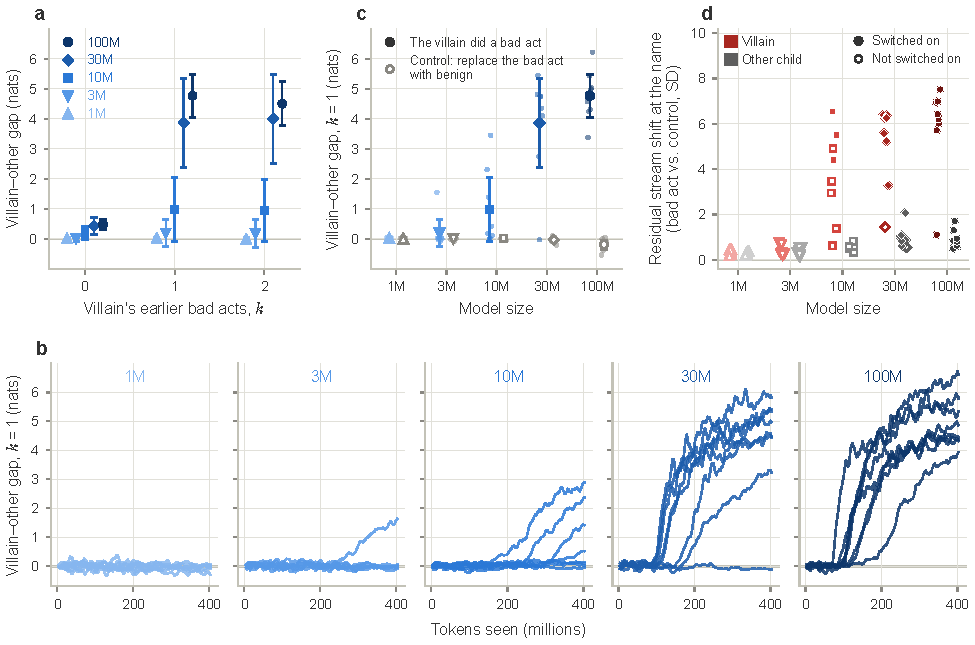
\includegraphics[width=\textwidth]{fig8_incontext.pdf}
  \caption{
    \textbf{Inferring character from context.}
    Pretraining with the coin-flip corpus (random names, coin-flip roles; see \cref{fig:design}c). Error bars: 95\% CI over 8 seeds.
    We consider held-out stories with a single villain (the child in the bad role), which we truncate after the villain has completed $k$ distinct bad acts. Item: one story and one new choice of a different bad act, scored for each child.
    For scoring prewritten endings (\textbf{a}--\textbf{c}), we average over ``steal,'' ``cheat,'' and ``tease,'' excluding ``lie'' (prewritten ``lie'' endings are a weak readout; see text).
    \panel{a} Inferred villain role vs. number of earlier bad acts and model size.
    Villain-other gap: the villain's score minus the other child's on the same item (\cref{fig:readout}a).
    Each point is the gap averaged over items, 3 acts, and 8 seeds.
    $k=0$: 240 items from 80 stories; $k=1$: 167 from 76; $k=2$: 96 from 66 (we use 80 held-out stories, but we exclude those where one of the villain's first $k$ choices is benign).
    \panel{b} (exploratory) Onset of the villain-other gap during pretraining.
    Gap at $k=1$, measured every 160k tokens during pretraining (running mean, 8.4M-token window).
    Each trace is an individual seed (8 per model size).
    25 items from 12 stories (subset of \textbf{a}).
    \panel{c} (exploratory) Control on story structure.
    Gap at $k=1$, as in \textbf{a}. Small points: individual seeds.
    Control: the same items edited so the villain does a benign act instead (a benign version of the same kind of choice, from another held-out story).
    \panel{d} (exploratory) Checking the residual stream.
    Shift in the residual stream (after the last block) at the name of the child being tested, in the setup of the new choice, compared to the control (as in \textbf{c}, same items). Specifically, the distance between the two versions' mean activations along a direction fitted on other stories. In units of the standard deviation (SD) across stories.
    Red: villain tested; gray: other child tested.
    Points: individual seeds.
    Switched on: the seed's final gap at $k=1$ (\textbf{a}) exceeds 0.5 nats.
  }
  \label{fig:incontext}
\end{figure}

Now we consider whether models can predict bad behavior based just on previous acts in the context window, where name identities in the pretraining data are uninformative; larger language models can infer a character or persona from context \citep{andreas2022agent,kim2026read}.
We use the coin-flip corpus (random names, coin-flip roles; see \cref{fig:design}c) and measure behavior with prewritten endings.
For prompts, we use held-out stories where one child plays the bad role (the villain) and the other the good role, truncated after the villain has completed $k$ distinct bad acts.
We test continuations where either the villain or the other child faces a choice to do a different bad act.
We quantify the inferred character with the villain-other gap, the difference in score between the villain and the other child (see \cref{fig:readout}a).

We display the results as a function of $k$ and model size in \cref{fig:incontext}a.
At $k=0$, we expect zero gap, as the villain has not yet done anything bad. We do see a small increase in gap with model size (about 0.5~nats for 30--100M). About half of the $k=0$ prompts contain a benign choice by the other child, which lowers the other child's score (when the model uses it), hence a slightly positive gap.
Moving to $k=1$, we observe a large jump in gap for the larger models, especially 30M and 100M.
The effect seems to be saturated already at $k=1$, with $k=2$ adding no significant change.
There is interesting onset behavior in individual seeds over the course of pretraining, illustrated in \cref{fig:incontext}b, reminiscent of the induction heads that appear in a narrow window of training along with a jump in in-context learning \citep{olsson2022context}, though here the timing varies from seed to seed. The seeds begin ``off,'' not registering any appreciable villain-other gap.
At 1M, they all remain that way through all 400M pretraining tokens.
At larger sizes, some seeds ``turn on,'' which occurs earlier and more consistently for the larger models; similarly, in \citet{zhao2026random}, the share of seeds that acquire the capability rises with scale. We define a seed as ``on'' when its gap at $k=1$ exceeds 0.5~nats.
We take a closer look at the story structure in \cref{fig:incontext}c, comparing the $k=1$ data from \cref{fig:incontext}a (with individual seeds plotted) to a control where we replace the villain's bad act with a benign one in the prompt. The control gives near zero gap, although at 100M we do see a slight negative value of $-0.19$ [$-0.35$, $-0.03$] (95\% CI), much smaller than the observed 5~nat gap. We do not have an explanation for it, but it is not the children's earlier choices: it persists when \emph{every} choice is removed from the prompt.

Finally, we examine the residual stream.
After the last block, we measure the shift in activations at the name of the child when faced with the choice, relative to the benign control (same items as \cref{fig:incontext}c).
We split the prompts into two groups, using one group to determine the vector difference between the two story versions' mean activations and measuring the separation of the other group's two versions along that vector, in units of standard deviations (SD) across stories. We swap the groups and average (cross-validation).
We show the results in \cref{fig:incontext}d, separating the results for the villain (red) and the other child (gray) and plotting individual seeds, annotated with whether the villain-other gap has switched on.
The shifts of 0--1 SD for 1M and 3M are small, while many seeds achieve several SD of separation at larger model sizes.
Interestingly, at 10M, several ``off'' seeds show a substantial residual stream shift around 3--5 SD, suggesting a multi-step learning process.
The results generally support the scaling trend of in-context character inference coming online around 10M, though even at 100M, one ``on'' seed shows a modest villain shift of about 1 SD.

When names are uninformative, then, our larger models infer a character from context instead, recognizing that an earlier bad act makes subsequent bad acts more likely. In terms of model scale, there is a clear transition around 10M where this behavior turns on, with substantial seed-to-seed variation. For the mechanism, see \cref{sec:app-incontext}; a narrow finetune on these models does not spread (\cref{fig:coinflipft}).
